\documentclass[12pt, letterpaper]{article}

% Packages
\usepackage[utf8]{inputenc}
\usepackage[sorting=none]{biblatex}
\usepackage{amsmath}
\usepackage{tabularx}
\usepackage{graphicx}
\usepackage{csquotes}
\usepackage{float}
\usepackage[normalem]{ulem}
\usepackage{subcaption}
\usepackage{authblk}
\usepackage{array}

% Bibliography
\addbibresource{./bib/Ma_2020.bib}
\addbibresource{./bib/rnn-effectiveness.bib}
\addbibresource{./bib/Understanding_LSTM.bib}
\addbibresource{./bib/Ramamoorthy.bib}
\addbibresource{./bib/Ramamoorthy2.bib}

% Parragraph formatting
\setlength{\parskip}{1em}

\title{Implementación de un Chatbot utilizando una Red Neuronal Seq2Seq}

\author[1]{Nathaniel Calderón González}
\author[2]{Ernesto Mancebo Tavárez}
\affil[1]{MULCIA, Universidad de Sevilla, Sevilla, España}

\date{Junio 2020}

\begin{document}
    \begin{titlepage}
        \maketitle
        \begin{abstract}
            A continuación se presenta la memoria de un estudio de la implementación de un chatbot mediante el uso de una Red Neuronal bajo la arquitectura Seq2Seq, la misma es entrenada utilizando el Corpus de mensajes del microblog Twitter.
        \end{abstract}
    \end{titlepage}

    \section{Objeto de Estudio}
    \section{Estado del Arte}
    \begin{table}[htb]
        \centering
        \resizebox{\textwidth}{!}{
            \begin{tabular}{l|p{0.4\textwidth}|p{0.7\textwidth}}
                \hline
                \textbf{Implementación} & \textbf{Ventajas} & \textbf{Desventajas} \\
                \hline
                K-Nearest Neightbor & Puede determinar anomalías y fácil de implementar. & Alto consumo de recursos. \\
                Redes Neuronales Artificiales & Aprende patrones de transacciones previas y detecta fraudes en tiempo real. & Se debe de estudiar la técnica a utilizar. \\
                Arboles de Desición & Maneja patrones no lineales. & Igual que las RNA, existen varias técnicas por lo que hay que estudiar cuál conviene. \\
                Outlier Detection Method & Consume menos recursos que otras técnicas y puede trabajar con data en línea (online) & No es tan preciso como otros métodos. \\
                Aprendizaje Profundo & Estudia y extrae patrones de grandes conjuntos de datos. & Es utilizado mayormente en procesamiento de imágenes y del lenguaje, por lo que para este campo hay poca información. \\
                \hline
            \end{tabular}
        }
        \caption{Estado del arte para implementaciones de Chatbots.}
    \end{table}

    \section{Redes Seq2Seq}
    \subsection{Redes Recurrentes - RNN}
    A medida que se analizan estructuras tales como una fotografía, todo el contenido es capturado a la vez y el mismo no cambia a través del tiempo mas no toda la información es analizada de esta manera; existen estructuras donde se depende de la evolución de la misma para conocer su significancia, es decir, se necesita conocer en un determinado punto sus valores previos, es por ello que necesitamos herramientas que traten la información de manera secuencial [Cita Naranjo].

    Para solventar esto se tienen las Redes Neuronales Recurrentes (RNN) las cuales son diseñadas para el análisis de secuencias. Estas redes se caracterizan por lo siguiente:
    
    \begin{itemize}
        \item Comparten parámetros.
        \item Capaces de procesar secuencias de distintas longitudes.
        \item Detectan información relevante que pueden aparecer en distintas posiciones de la secuencia.
    \end{itemize}
    A modo de ejemplificar la última característica de estas redes se tiene \emph{"El 23 de Enero salí a pasear"} o \emph{"Salí a pasear el 23 de Enero"}. 

    Las RNN no conocen el significado de los símbolos que procesan, éstas infieren en el significado a partir de la extructura de la secuencia y la posición de los símbolos. Por otro lado, una RNN es capáz de lograr todo lo mencionado por el hecho de que tales redes tienen un estado al que en ocasiones se le puede escuchar referir como \emph{memoria}.

    El estado o memoria de tal red se logra a partir del hecho de que una RNN son redes con bucles dentro de ella.

    \begin{figure}[H]
        \centering
        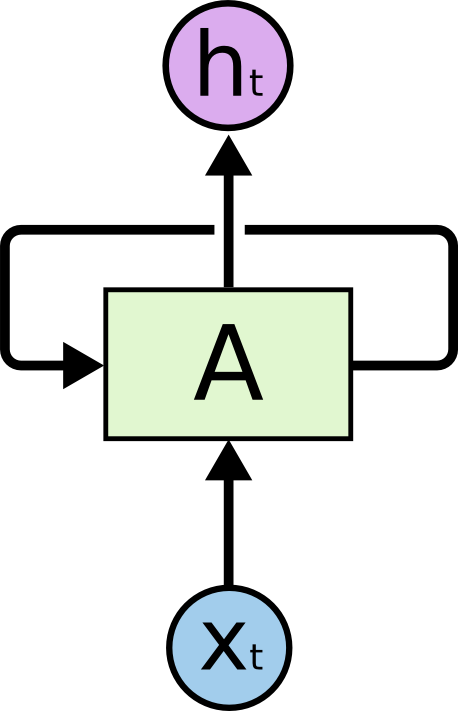
\includegraphics[width=\linewidth]{img/RNN-rolled.png}
        \caption{Ilustración de una RNN.}
    \end{figure}

    En la representación se tiene un trozo de red $A$ la cual toma como entrada un $x_t$ y emite un valor $h_t$, de este modo, utilizando el bucle mencionado, la información pasa al siguiente paso dentro de la red. Dicho ya esto, podemos ilustrar una red recurrente como una red con múltiples copias de sí misma\cite{Understanding_LSTM}.

    \begin{figure}[H]
        \centering
        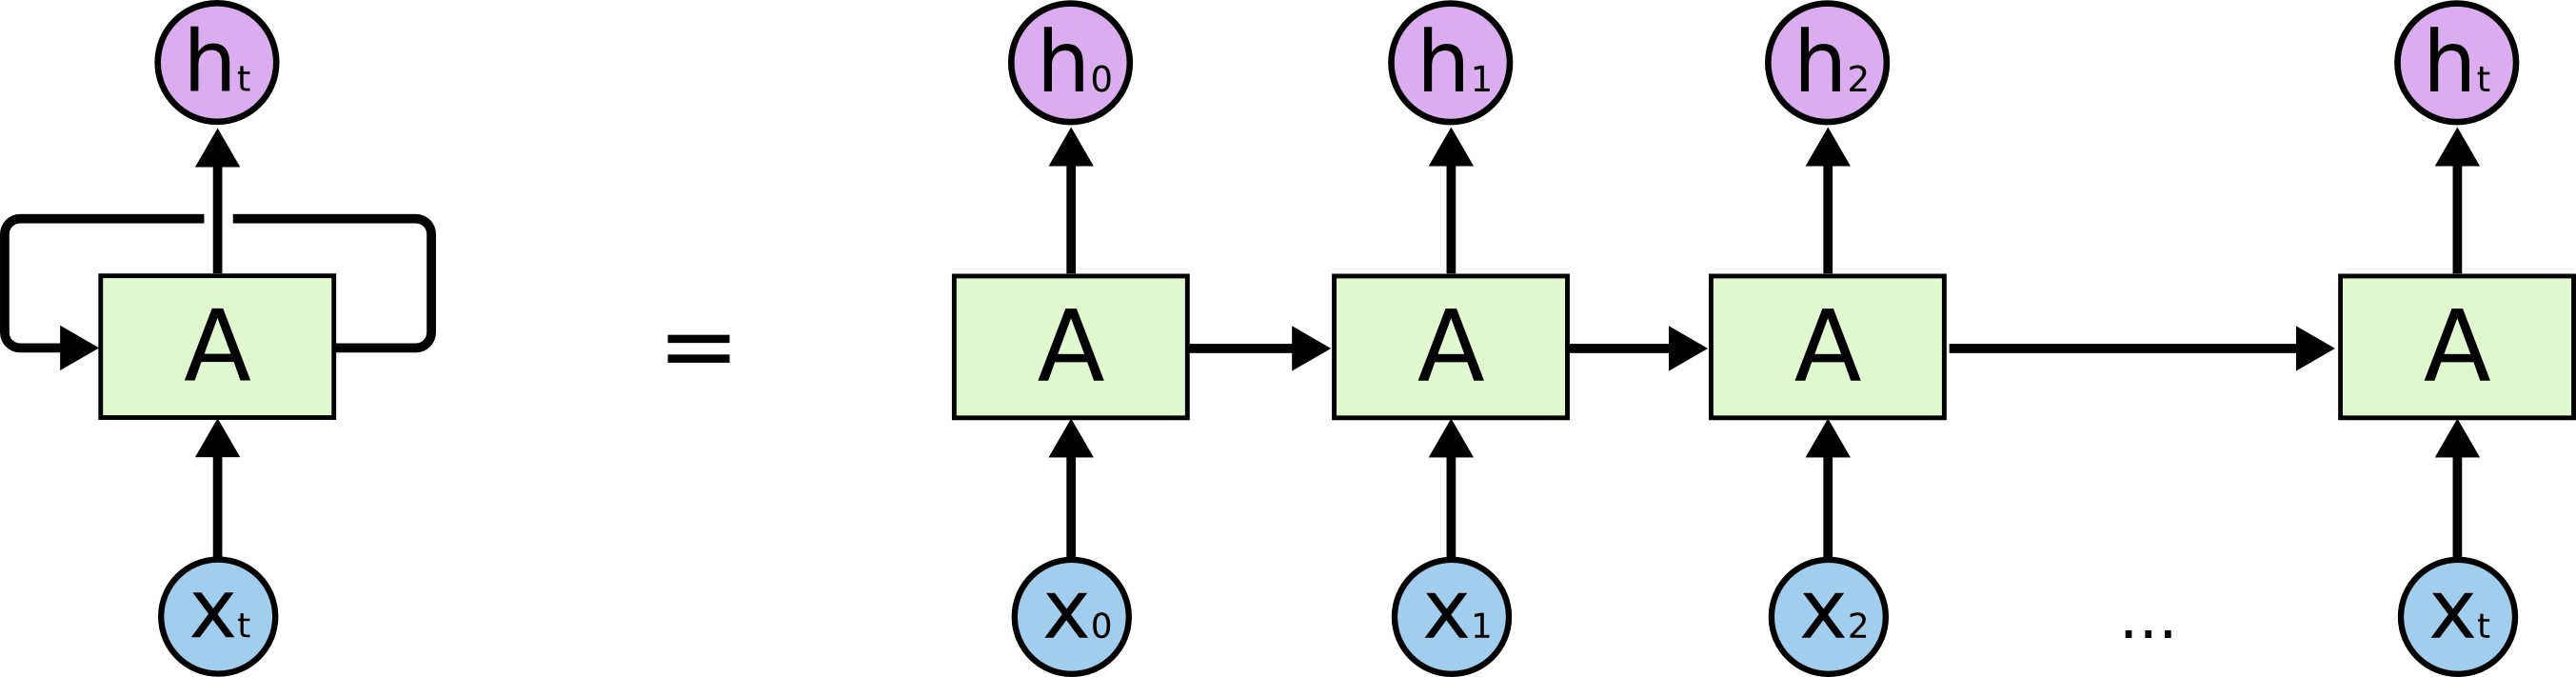
\includegraphics[width=\linewidth]{img/RNN-unrolled.png}
        \caption{Ilustración de la evolución de una RNN a través del tiempo $t$.}
    \end{figure}
    
    Este comportamiento en secuencia es lo que enlaza las RNN con secuencias y listas, por ellos, tales redes son exitosas para problemas de reconocimiento de voz, modelado del lenguaje, traducción, contextualización de imágenes y otras aplicaciones relacionadas\cite{rnn-effectiveness}.

    \subsection{Redes Long Short-Term Memory - LSTM}
    Una variante las RNN capáz de aprender a partir de dependencias a largo plazo es la Long Short Term Memory, muchas veces llamadas tan solo LSTM.
    
    Las LSTM fueron diseñadas con la intención de evitar problemas de dependencia a largo plazo, con la naturaleza de recordar información por un largo período de tiempo.
    
    La estructura interna de una LSTM varía un poco de una RNN regular, donde en vez de tener una única capa, tiene cuatro y cada una interactúa de un modo distinto.

        \begin{figure}[H]
            \centering
            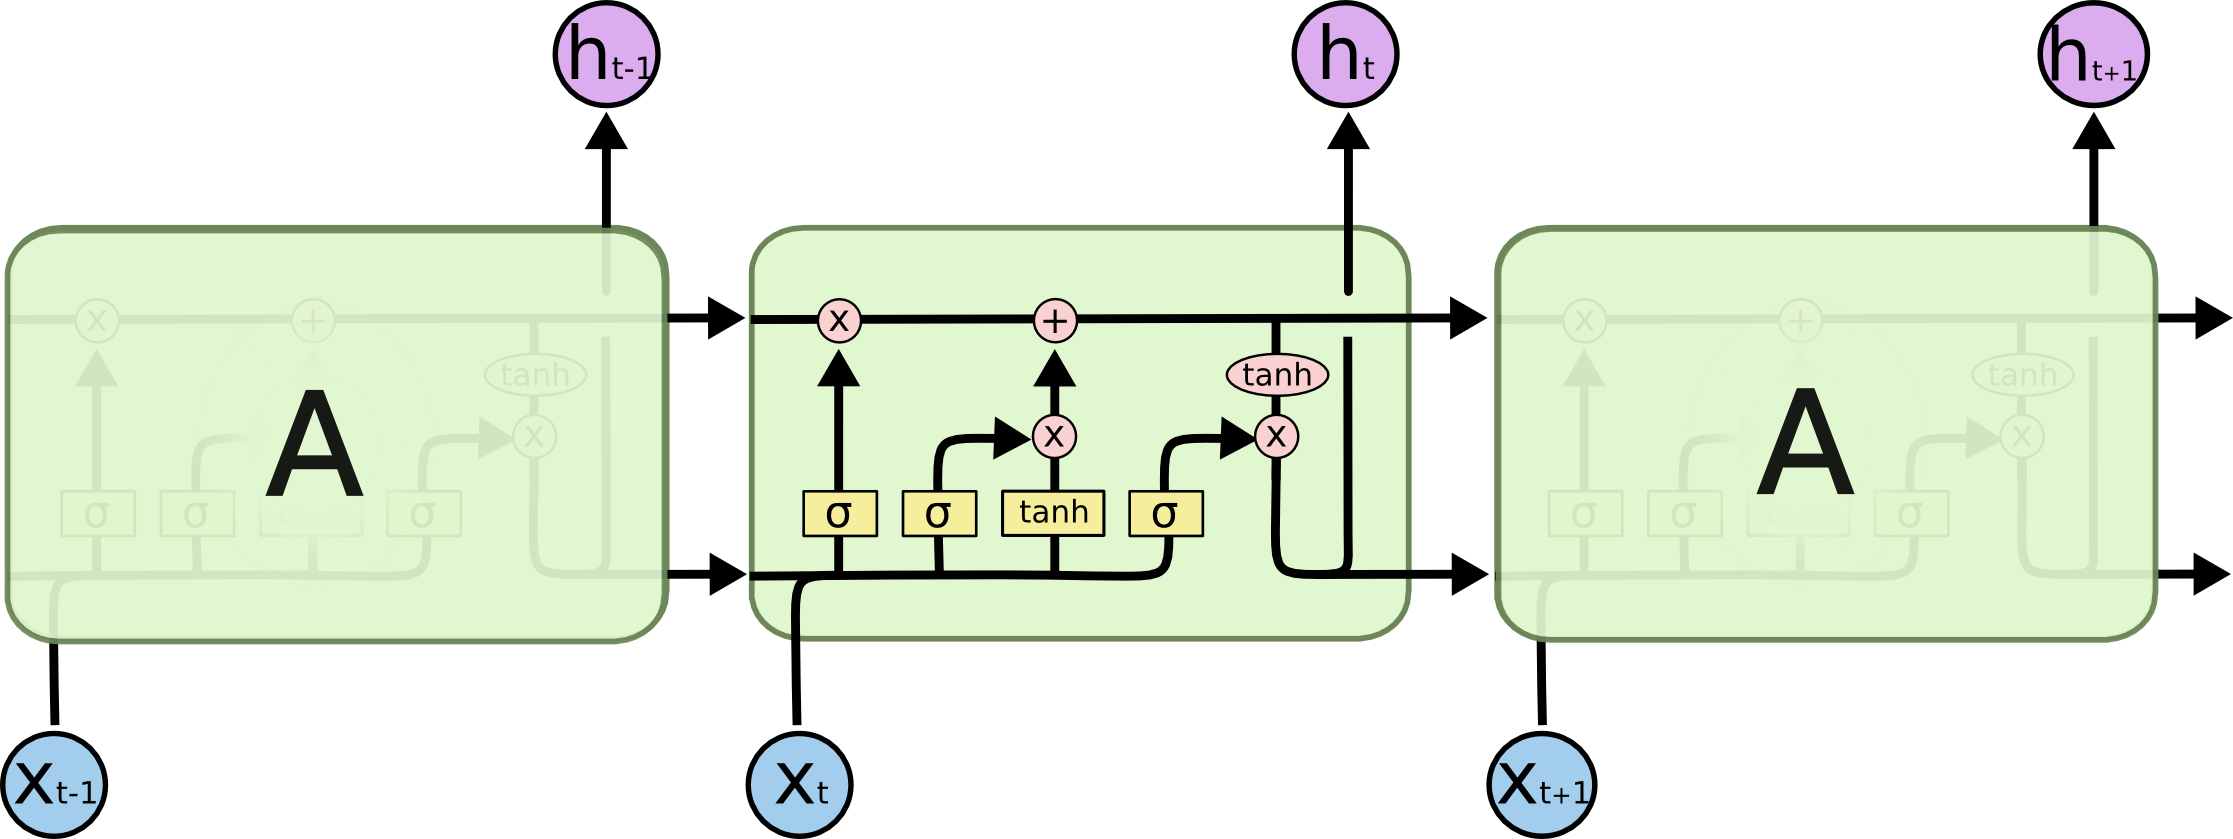
\includegraphics[width=\linewidth]{img/LSTM3-chain.png}
            \caption{Ilustración de una red LSTM.}
        \end{figure}

        A continuación tenemos una radiografía de lo que conforma una red LSTM.
        \begin{figure}[H]
            \centering
            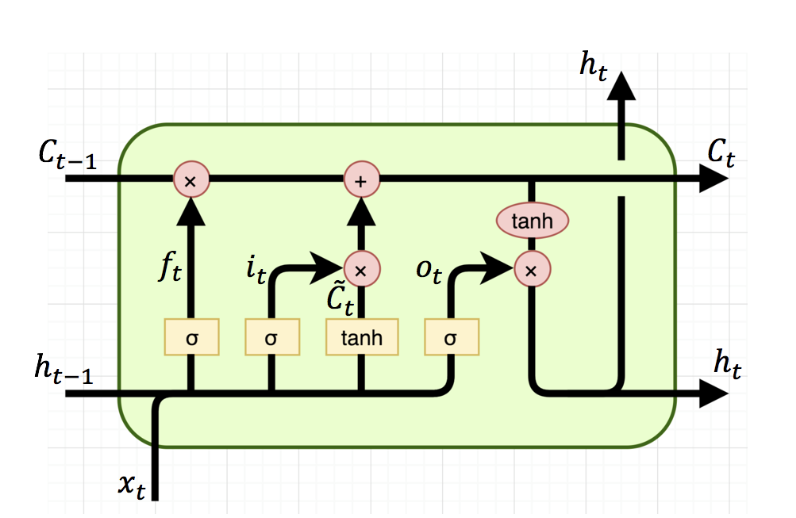
\includegraphics[width=\linewidth]{img/LSTM3-cell-A.png}
            \caption{Composición interna de una LSTM.}
        \end{figure}

        Como se puede apreciar la red está compuerta por varias compuertas (\emph{gates}) los cuales tienen la tarea de agregar o eliminar data al estádo de la celda. Cada celda es controlada por una capa que se apoya en la función sigmoide ($\sigma$) y la operación producto. Es preciso resalta que la función sigmoide retorna un valor entre cero y uno, siendo cero \emph{no pase información} y uno \emph{pase toda la información}. Finalmente, una LSTM contiene tres compuertas $\sigma$ descritas de la siguiente manera:

        \begin{itemize}
            \item $f_t$ o \emph{"Puerta del Olvido"}, decide qué dato se debe de descartar en el estado de la celda tras observar los valores de $h_{t-1}$ y $x_t$, retornando un número entre cero y uno para cada valor en el estado $C_{t-1}$.
            \begin{equation}
                f_t = \sigma(W_f\cdot{[h_{t-1},x_t]} + b_f) 
            \end{equation}

            En un problema de modelado del lenguaje, $f_t$ trataría de predecir la siguiente palabra a partir de las anteriores. De modo que para un primer sujeto trataría de inferir en su género, sin embargo, para un siguiente sujeto la celda olvidaría el género del primero y tratára de identificar el del segundo.

            \item En el siguiente paso se decide qué información se debe de persistir en la celda tras dos pasos, primero la capa sigmoide llamada \emph{"Capa Puerta de Entrada"} la cual decide qué valor se actualiza seguido de la creación de nuevos candidatos tras una capa que utiliza la Tangente Hiperbólica crea un vector de nuevos candidatos $\tilde{C_t}$. Estas luego se combinan y actualizan el estado de la celda en cuestión.
            \begin{equation}
                \begin{aligned}
                    i_t &= \sigma(W_i\cdot{[h_{t-1}, x_t]} + b_i) \\
                    \tilde{C}_t &= \text{tanh}(W_c\cdot{[h_{t-1}, x_t]} +b_C)
                \end{aligned}
            \end{equation}

            Siguiendo la línea del modelado del lenguaje, para el segundo sujeto en la secuencia se actualizaría su género en la celda reemplazando así el género del sujero previo.

            \item En este tercer paso se produce la actualización del estado anterior $C_{t-1}$ en $C_t$, logrado esto en los pasos previos. Primero se olvidan los estados previos mediante $f_t$, se computa los nuevos valores mediante $i_t*\tilde{C_t}$ dándonos esto el nuevo valor para el estado $C_t$. 
            \begin{equation}
                    C_t = f_t* C_{t-1} + i_t*\tilde{C_t}
            \end{equation}

            \item Finalmente se procede a emitir un valor de salida para la celda, mas éste valor debe de ser filtrado. El primer paso es a través de una sigmoide se decide qué se debe de emitir $o_t$, luego el estado actual de la celda $C_t$ es evaluado por una Tangente Hiperbólica y finalmente multiplicado por el resultado de $o_t$, filtrándose así la salida\cite{Understanding_LSTM}.

            \begin{equation}
                \begin{aligned}
                    o_t &= \sigma(W_o\cdot{[h_{t-1}, x_t]} + b_o) \\
                    h_t &=  o_t*\text{tanh}(C_t)
                \end{aligned}
            \end{equation}
        \end{itemize}

    \subsection{Redes Seq2Seq}
    Una implementación Seq2Seq consiste en dos redes recurrentes (RNN) enlazadas, una siendo codificadora y la otra decodificadora. La tarea de la codificador es leer una secuencia de entrada y emitir un contexto a partir del último estado oculto $h_t$ a partir de lo que considere importante en la secuencia de entrada. Posteriormente se tiene una red decodificadora la cual utiliza una función softmax sobre el vocabulario a utilizar para así emitir una secuencia de salida\cite{Ramamoorthy}\cite{Ramamoorthy2}.

    \begin{figure}[H]
        \centering
        \includegraphics[width=\linewidth]{img/Seq2Seq.png}
        \caption{Comportamiendo de una red Seq2Seq.}
    \end{figure}

    Se aprecia en la parte central de un modelo Seq2Seq lo que se conoce como \emph{Though Vector} o vector de pensamiento, el cuál representa la intención de la secuencia de entrada y a partir de aquí la sección decodificadora del modelo genera una secuencia a emitir, símbolo tras símbolo, palabra en este caso, donde cada símbolo es influenciado por el anterior.

    \section{Corpus}
    El corpus utilizado para entrenar esta red corresponde a un conjunto de más de 700 mil mensajes procedentes de la red social Twitter. Este corpus es provisto por el respositorio chat\_corpus\cite{Ma_2020} donde detalla que para las líneas impares corresponden a \emph{tweets} y las líneas pares corresponden a respuestas al \emph{tweet} predecesor.

    \section{Implementación}

    \subsection{Retos de la Implementación}
    Existen varios retos para el modelo Seq2Seq y uno de ellos es la variabilidad de la longitud de la secuencias, pues la longitud de las secuencias de entrada a procesar es indiscutiblemente variable. Otro problema es la dimención del vocabulario a utilizar, pues es ineficiente aplicar una función softmax a cada palabra de nuestro vocabulario\cite{Ramamoorthy}.

    \subsection{Relleno de Oraciones (Padding)}
    \subsection{Empaquetado (Bucketing)}
    \subsection{Contextualización de Palabras (Word Embedding)}
    \subsection{Attention Mechanism}
    \subsection{Código}

    \section{Resultados}
    \section{Conclusiones}

    \pagebreak
    \printbibliography[title={Bibliografía}]
\end{document}